%=============================
%  PRIMER CAPITULO
%=============================
\chapter{Introducción}
\label{cap1}

En este capitulo el autor debe plantear de forma clara el tema que ira a desarrollar en su investigación. El autor debe describir el estado de arte de su investigación de forma breve. Por ejemplo, debe considerar los trabajos anteriores que realizaron otros autores sobre el tema de investigación, resaltando sobre todo los resultados encontrados.\\

Para la citación de los trabajos de investigación el autor tendrá las siguientes opciones que se muestran a manera de ejemplo: \cite{tabari2020} mostró que el impacto del cambio climático esta afectando las tasas de precipitación, además encontraron que hay un aumento en la frecuencia de ocurrencia de precipitaciones extremas que están ocasionando inundaciones en muchas ciudades alrededor del mundo.\\ 

Otra forma de citar es: Los impactos del cambio climático son observados en las tasas de precipitación, y estos están asociados a un aumento en la frecuencia de ocurrencia de precipitaciones extremas, los cuales están generando inundaciones en varias ciudades alrededor del mundo \citep{tabari2020}. A continuación se muestra un ejemplo de como citar una Figura~\ref{fig01} de forma automática a lo largo del documento.\\

\begin{figure}[!ht]
\centering
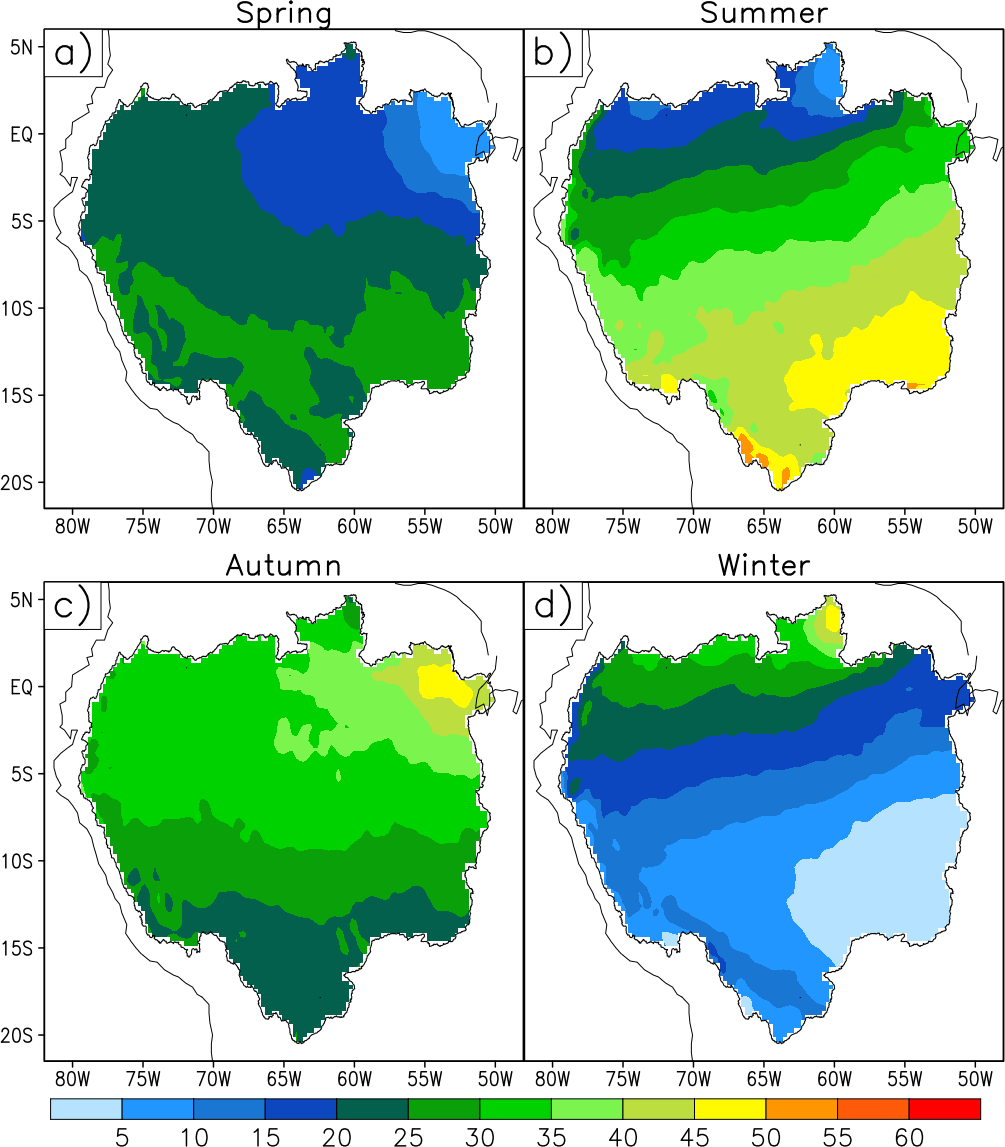
\includegraphics[width=0.55\textwidth]{pre-amz.png}
\caption{Contribución de la precipitación estacional (\%) sobre la cuenca Amazónica para el periodo 1981-2010, realizado con datos de reanálisis ERA5.}
%\raggedright Fuente: Adaptado de \cite{greenwade93}.
\label{fig01}
\end{figure}


Ahora se muestra una opción de como citar varios trabajos de investigación. Muchos estudios de modelado muestran una reducción de la precipitación y un aumento de la temperatura en la región tropical en el futuro, siendo que estos cambios son mas intensos en el escenario más pesimista (RCP8.5)~\citep{reboita14,reboita21,blazquez20,llopart20}.

Otra forma de de insertar Figuras en el contenido del documento es cuando se toma como referencia una figura de un trabajo de investigación anterior. La Figura~\ref{fig02} muestra el dominio de simulación realizado con el modelo regional. La Figura~\ref{fig03} muestra otra alternativa de citar adecuadamente la figura de otros autores. 

\begin{figure}[htbp]
\centering
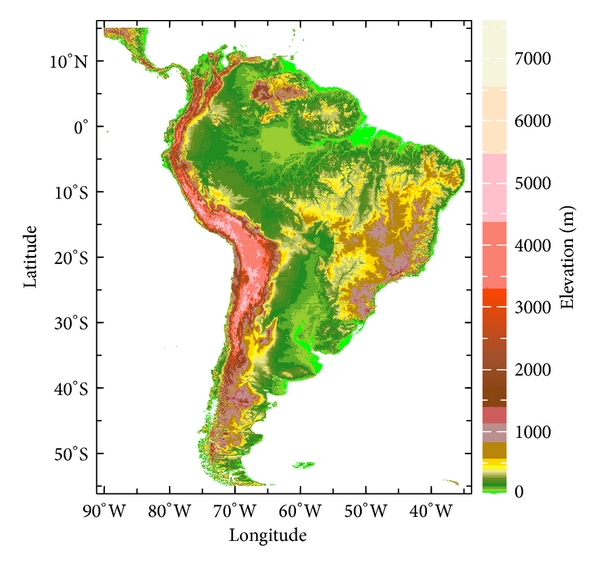
\includegraphics[width=0.8\textwidth]{topografia.jpg}
%\raggedright \textbf{Fuente:} Adaptado de \cite{solman2013}.
%\centering \textbf{Fuente:} .
\captionsource{Topografía (m) de América del Sur, generado con datos de ETOPO5.}{Obtenido de \cite{solman2013}.}
\label{fig02}
\end{figure}


\begin{figure}[!ht]
\centering
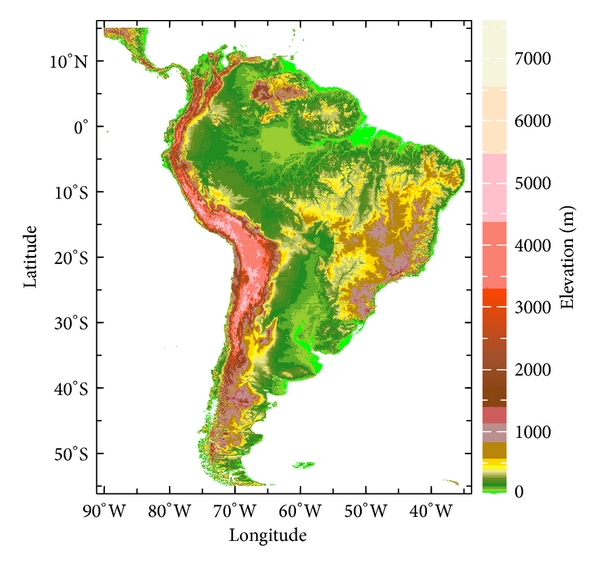
\includegraphics[width=1.0\textwidth]{topografia.jpg}
\vspace{-1.0cm}
\caption{Topografía de América del Sur.}
%\raggedright \textbf{Fuente:} Adaptado de \cite{solman2013}
\centering \textbf{Fuente:} Adaptado de \cite{solman2013}.
\label{fig03}
\end{figure}

La ecuación \(x^2 + y^2 = z^2\) muestra el teorema de Pitágoras. Otra forma de escribir ecuaciones en intermedio de los párrafos es de la siguiente manera: $(a+b)^2 = a^2 + 2ab + b^2$. La ecuación~\ref{eq1} muestra el resultado del calculo de la integral cerrada. 

\begin{equation}
\oint_{a}^{b} = \sqrt{x^2+1}
\label{eq1}
\end{equation}

También se puede insertar ecuaciones a lo largo del texto sin numeración, para ello solo debe seguir el procedimiento del siguiente ejemplo:\newline

\begin{equation*}
\oint_{a}^{b} = \sqrt{x^2+1}
\label{eq2}
\end{equation*}

Como se observa la ecuación inmediata superior no tiene la numeración. A continuación se muestra algunas alternativas de como el usuario puede centrar las ecuaciones con múltiples lineas. 

\begin{gather}
((a+b)^2 = a^2 + 2ab + b^2\\
(a-b)^2 = a^2 - 2ab + b^2\\
(a+b)(a-b) = a^2 - b^2
\end{gather}

\begin{align}
((a+b)^2& = a^2 + 2ab + b^2\\
(a-b)^2& = a^2 - 2ab + b^2\\
(a+b)(a-b)& = a^2 - b^2
\end{align}


Las Tablas también sarán insertadas a lo largo del texto, para ello ver los siguientes ejemplos:\newline


\begin{table}[!h]
\begin{center}
\begin{tabular}{| l | c | c | c | c | }
\hline
\multicolumn{5}{ |c| }{Valores promedios de precipitación} \\ \hline
\textbf{Ciudades} & \textbf{Verano} & \textbf{Otoño} & \textbf{Invierno} & \textbf{Primavera} \\ \hline
Huancayo & 80 mm & 70 mm & 10 mm & 35 mm \\
La Mar & 85 mm & 65 mm & 5 mm & 93 mm \\
Coricancha & 35 mm & 30 mm & 2 mm & 45 mm \\
Sucre & 65 mm & 45 mm & 10 mm & 20 mm \\ \hline
\end{tabular}
\caption{Valores de precipitación para tres ciudades del Perú en escala estacional durante el periodo 2000-2010.}
\label{tabla1}
\end{center}
\end{table}


La Tabla~\ref{tabla2} muestra la precipitación acumulada para las principales estaciones meteorológicas del sur de Lima. En esta tabla se puede observar que la estación 4 recibe la mínima precipitación. 

Lorem ipsum dolor sit amet, consectetur adipiscing elit. Aliquam ultricies lacinia euismod. Nam tempus risus in dolor rhoncus in interdum enim tincidunt. Donec vel nunc neque. In condimentum ullamcorper quam non consequat. Fusce sagittis tempor feugiat. Fusce magna erat, molestie eu convallis ut, tempus sed arcu. Quisque molestie, ante a tincidunt ullamcorper, sapien enim dignissim lacus, in semper nibh erat lobortis purus. Integer dapibus ligula ac risus convallis pellentesque.

\begin{table}[!h]
\centering
\begin{tabular}{|c|c|c|c|c|}
\hline
\textbf{Estación 1} & \textbf{Estación 2} & \textbf{Estación 3} & \textbf{Estación 4} & \textbf{Estación 5} \\ \hline
20    & 25     & 22     & 16     & 87      \\ \hline
30    & 45     & 65     & 22     & 57      \\ \hline
10    & 12     & 60     & 1      & 12      \\ \hline
\end{tabular}
\caption{Datos de precipitación acumulado (mm) para cinco estaciones meteorológicas.}
\label{tabla2}
\end{table}

Lorem ipsum dolor sit amet, consectetur adipiscing elit. Aliquam ultricies lacinia euismod. Nam tempus risus in dolor rhoncus in interdum enim tincidunt. Donec vel nunc neque. In condimentum ullamcorper quam non consequat. Fusce sagittis tempor feugiat. Fusce magna erat, molestie eu convallis ut, tempus sed arcu. Quisque molestie, ante a tincidunt ullamcorper, sapien enim dignissim lacus, in semper nibh erat lobortis purus. Integer dapibus ligula ac risus convallis pellentesque. Lorem ipsum dolor sit amet, consectetur adipiscing elit. Aliquam ultricies lacinia euismod. Nam tempus risus in dolor rhoncus in interdum enim tincidunt. Donec vel nunc neque. In condimentum ullamcorper quam non consequat. Fusce sagittis tempor feugiat. Fusce magna erat, molestie eu convallis ut, tempus sed arcu. Quisque molestie, ante a tincidunt ullamcorper, sapien enim dignissim lacus, in semper nibh erat lobortis purus. Integer dapibus ligula ac risus convallis pellentesque.

Lorem ipsum dolor sit amet, consectetur adipiscing elit. Aliquam ultricies lacinia euismod. Nam tempus risus in dolor rhoncus in interdum enim tincidunt. Donec vel nunc neque. In condimentum ullamcorper quam non consequat. Fusce sagittis tempor feugiat. Fusce magna erat, molestie eu convallis ut, tempus sed arcu. Quisque molestie, ante a tincidunt ullamcorper, sapien enim dignissim lacus, in semper nibh erat lobortis purus. Integer dapibus ligula ac risus convallis pellentesque. Lorem ipsum dolor sit amet, consectetur adipiscing elit. Aliquam ultricies lacinia euismod. Nam tempus risus in dolor rhoncus in interdum enim tincidunt. Donec vel nunc neque. In condimentum ullamcorper quam non consequat. Fusce sagittis tempor feugiat. Fusce magna erat, molestie eu convallis ut, tempus sed arcu. Quisque molestie, ante a tincidunt ullamcorper, sapien enim dignissim lacus, in semper nibh erat lobortis purus. Integer dapibus ligula ac risus convallis pellentesque. 

\section{Motivación}
Escriba aquí la motivación de su trabajo de investigación si lo tuviera ....


\section{Objetivo}
Escriba aquí el objetivo de su trabajo de investigación... 

\subsection{Objetivos específicos}
Escriba aquí sus objetivos de su investigación si los tuviera.... 
